\documentclass[hyperref={colorlinks=true,linkcolor=blue,citecolor=blue}]{beamer}
\usepackage{amsmath}
\usepackage{amssymb}
\usepackage{amsfonts}
\usepackage{tikz}
\usepackage[round]{natbib}
\usepackage{pifont}
%\usetheme{boadilla}
\newcommand{\cmark}{\ding{51}}
\newcommand{\xmark}{\ding{55}}
\DeclareMathOperator{\pr}{Pr}
\DeclareMathOperator{\e}{E}
\DeclareMathOperator*{\argmax}{argmax}
\DeclareMathOperator*{\argmin}{argmin}
\newtheorem{prop}{Proposition}
\newtheorem{corr}{Corollary}
\newtheorem{assn}{Assumption}
\newtheorem{refinement}{Refinement}
\usetikzlibrary{arrows,automata,fit}
\renewcommand{\qedsymbol}{$\blacksquare$}
\renewcommand{\arraystretch}{2}	
\usetikzlibrary{arrows,automata,fit}
\setbeamersize{description width=0.25in}
\title{Clarifying by Discretizing}
\author{Jordan Martel$^{\dagger}$, Edward Van Wesep$^{\dagger}$, Robert Van Wesep$^{\ddagger}$\\{\small University of Colorado at Boulder$^{\dagger}$, Unaffiliated$^{\ddagger}$}}
\date{FIRS 2018}
\begin{document}
\maketitle
%%%%%%%%%%%%%%%%%%%%
%%% INTRODUCTION %%%
%%%%%%%%%%%%%%%%%%%%
\begin{frame}{Research Question}
\begin{center}
\textbf{Why do people discretize their communication?}
\end{center}
\vspace{.25in}
\pause
Examples of cheap, discrete messages:
\begin{itemize}
\item Bond ratings (AAA,$\ldots$,D)
\item Analysts' recommendations (Strong Buy, Buy, Hold, Sell, Strong Sell)
\item Course grades (A,$\ldots$,F)
\item Weather advisories (Tornado Watch, Tornado Warning)
\item Film and restaurant reviews ($\bigstar\bigstar\bigstar,\ldots,\bigstar$)  
\end{itemize}
\end{frame}

%%%%%%%%%%%%%%%%%%%%%%%%%%%%%%%%%%%%%%%%%%%
%%% OUR RESULT AND CLASSICAL CHEAP TALK %%%
%%%%%%%%%%%%%%%%%%%%%%%%%%%%%%%%%%%%%%%%%%%
\begin{frame}{Our Result}
\begin{itemize}
\item Crawford and Sobel (1982): 
\begin{equation*}
\text{conflict of interest }\Rightarrow\text{ discrete messages}.
\end{equation*}
\item We show that the converse is false:
\begin{equation*}
\text{conflict of interest }\nLeftarrow\text{ discrete messages}.
\end{equation*}
\item How? If (1) the message space is bounded, and (2) messages are received with noise, then 
\begin{equation*}
\text{\underline{no} conflict of interest }\Rightarrow\text{ discrete messages}.
\end{equation*}
\item \textbf{Discrete messages less precise, but easier to interpret.}
\end{itemize}
\end{frame}

%%%%%%%%%%%%%%%%%%%%
%%% INTRODUCTION %%%
%%%%%%%%%%%%%%%%%%%%
\begin{frame}{Research Question}
\begin{center}
\textbf{Why do people discretize their communication?}
\end{center}
\vspace{.25in}
Examples of cheap, discrete messages:
\begin{itemize}
\item Bond ratings (AAA,$\ldots$,D)
\item Analysts' recommendations (Strong Buy, Buy, Hold, Sell, Strong Sell)
\item Course grades (A,$\ldots$,F)
\item Weather advisories (Tornado Watch, Tornado Warning)
\item Film and restaurant reviews ($\bigstar\bigstar\bigstar,\ldots,\bigstar$)  
\end{itemize}
\pause In practice, both discrete and continuous (different receivers?)
\end{frame}


%%%%%%%%%%%%%
%%% LITERATURE %%%
%%%%%%%%%%%%%
\begin{frame}{Literature}
\begin{itemize}
\item Cheap talk: Large
\item Interests aligned, but messaging is discrete by assumption: {\small Sobel (2012), Cremer, Garicano, and Prat (2007), Garicano and Prat (2011)}
\item Benevolent sender, optimal messages discrete, but receivers' interests are not aligned: {\small Agranov and Schotter (2012) and Crawford, Gneezy and Rottenstreich (2008)}
\item Electrical Engineering
\end{itemize}
\end{frame}

%%%%%%%%%%%%%%%%%
%%% THE MODEL %%%
%%%%%%%%%%%%%%%%%
\begin{frame}{The Model}
There are two players, sender $(\textit{Sally})$, and receiver $(\textit{Robert})$. 
\begin{flushleft}
\begin{description}
\item[$t_{0}$] The sender privately observes the state of the world, $q\sim U[0,1]$.
\item[$t_{1}$] The sender sends the receiver a costless message, $m(q)$.
\item[$t_{2}$] The receiver receives
\begin{equation}
\widetilde{m}(q)\equiv m(q)+\epsilon
\end{equation}
where $\epsilon\sim U[-\bar{\epsilon},+\bar{\epsilon}]$, $\bar{\epsilon}>0$, and (for ease of expo) $\text{mod}(1,\bar{\epsilon})=0$.
\item[$t_{3}$] The receiver takes an action $a(\widetilde{m})\in\mathbb{R}$, and payoffs are realized.  
\end{description}
\end{flushleft}
The sender and receiver have preferences over the receiver's action
\begin{align}
U^{S}(a,q,b)&\equiv-(a-(q+b))^{2}\\
U^{R}(a,q)&\equiv-(a-q)^{2}
\end{align}
where $b\geq0$ measures the degree of conflict.
\end{frame}

%%%%%%%%%%%%%%%%%%
%%% COMPARISON %%%
%%%%%%%%%%%%%%%%%%
\begin{frame}{Comparison}
\begin{center}
\begin{tabular}{l|ccc}
& Interests & Noise & Messages\\ \hline
Crawford and Sobel & $b>0$ & $\bar{\epsilon}=0$ & $\mathbb{R}$\\
Martel and $2\times$Van Wesep & $b=0$ & $\bar{\epsilon}>0$ & $[0,1]$
\end{tabular}
\end{center}
\begin{itemize}
\item Crawford and Sobel: conflicts of interests, no noise, unbounded message space. 
\item Martel and $2\times$Van Wesep: no conflicts of interests, noise, bounded message space. 
\end{itemize}
\end{frame}

%%%%%%%%%%%%%%%%%%%%%%%%%%%%%%%%%%%%%%%%
%%% CRAWFORD AND SOBEL (TITLE SLIDE) %%%
%%%%%%%%%%%%%%%%%%%%%%%%%%%%%%%%%%%%%%%%
\begin{frame}
\begin{center}
\textbf{CRAWFORD AND SOBEL}
\end{center}
\end{frame}

%%%%%%%%%%%%%%%%%%%
%%% PREFERENCES %%%
%%%%%%%%%%%%%%%%%%%
\begin{frame}{Preferences}
\begin{center}
\includegraphics[scale=.45]{ObjectiveFunctions}\\
For each $q$, the sender prefers that the receiver take a larger $a$. 
\end{center}
\end{frame}

%%%%%%%%%%%%%%%%%%%%%%
%%% CRAWFORD SOBEL %%%
%%%%%%%%%%%%%%%%%%%%%%
\begin{frame}{Crawford and Sobel}
\begin{center}
\includegraphics[scale=.45]{CrawfordSobel}\\
\textbf{Theorem.} Unique equilibrium features discrete messages.
\end{center}
\end{frame}

%%%%%%%%%%%%%%%%%%%%%%%%%%%%%%%%%%%%%%%%%%%%
%%% MARTEL AND VAN WESEPX2 (TITLE SLIDE) %%%
%%%%%%%%%%%%%%%%%%%%%%%%%%%%%%%%%%%%%%%%%%%%
\begin{frame}
\begin{center}
\textbf{MARTEL AND $2\times$VAN WESEP}
\end{center}
\end{frame}

%%%%%%%%%%%%%%%%%
%%% THE MODEL %%%
%%%%%%%%%%%%%%%%%
\begin{frame}{Martel, $2\times$Van Wesep}
\begin{enumerate}
\item \textit{The sender and receivers' preferences are the same.}
\begin{itemize}
\item Teams
\item Partnerships
\end{itemize}
\item \textit{The message space is bounded} (w.l.o.g. to $[0,1]$).
\begin{itemize}
\item Hitler $\leq$ CEO $\leq$ Mother Teresa
\end{itemize}
\item \textit{Messages are received with error.} 
\begin{itemize}
\item\textit{The panda eats, shoots and leaves.}
\item\textit{The new manager believes in collaborative problem-solving.}
\item\textit{Congress is unable to address budget problems.}
\item\textit{Ann wrote poignan essays in my class.}
\end{itemize}
\end{enumerate}
\end{frame}

%%%%%%%%%%%%%%%
%%% UTILITY %%%
%%%%%%%%%%%%%%%
\begin{frame}{Utility}
Given a message and action
\begin{align}
m(q)&:[0,1]\rightarrow[0,1]\\
a(\widetilde{m})&:[-\bar{\epsilon},1+\bar{\epsilon}]\rightarrow\mathbb{R}
\end{align}
The sender \underline{and} receivers' expected utility is 
\begin{equation}
E[U]=-\int_{0}^{1}{\left[\int_{-\bar{\epsilon}}^{\bar{\epsilon}}{|a(m(q)+e)-q|^{2}\cdot\frac{de}{2\bar{\epsilon}}}\right]dq.}
\end{equation}
\begin{itemize}
\item $|a(m(q)+e)-q|^{2}$ is the quadratic loss given error $e$, and state $q$.
\item Integrate over errors, $e\sim U[-\bar{\epsilon},\bar{\epsilon}]$.
\item Integrate over states, $q\sim U[0,1]$. 
\end{itemize}
\end{frame}

%%%%%%%%%%%%%%%%%%%%%%%%
%%% IDENTITY MESSAGE %%%
%%%%%%%%%%%%%%%%%%%%%%%%
\begin{frame}{Identity Message}
\begin{center}
\includegraphics[scale=.45]{IdentityMessagePlot}\\
Having received $\widetilde{m}_{0}$, the receiver infers that $q\in[q_{-}(\widetilde{m}_{0}),q_{+}(\widetilde{m}_{0})]$. 
\end{center}
\end{frame}

%%%%%%%%%%%%%%%%%%%%%%%
%%% IDENTITY ACTION %%%
%%%%%%%%%%%%%%%%%%%%%%%
\begin{frame}{Identity Action}
\begin{center}
\includegraphics[scale=.45]{IdentityActionPlot}\\
\textbf{Lemma 1.} $a^{*}(\widetilde{m})=(q_{-}(\widetilde{m}_{0})+q_{+}(\widetilde{m}_{0}))/2$. 
\end{center}
\end{frame}

%%%%%%%%%%%%%%%%%%%%%%
%%% IDENTITY ERROR %%%
%%%%%%%%%%%%%%%%%%%%%%
\begin{frame}{Identity Error}
\begin{center}
\includegraphics[scale=.45]{continuouserror}\\
The error, $|a(\widetilde{m})-q|$, is \underline{uniformly distributed} on this hexagon.
\end{center}
\end{frame}

%%%%%%%%%%%%%%%%%%%%%%%%
%%% DISCRETE MESSAGE %%%
%%%%%%%%%%%%%%%%%%%%%%%%
\begin{frame}{Discrete Message}
\begin{center}
\includegraphics[scale=.45]{DiscreteMessagePlot}\\
There is no uncertainty about which message was sent!
\end{center}
\end{frame}

%%%%%%%%%%%%%%%%%%%%%%%
%%% DISCRETE ACTION %%%
%%%%%%%%%%%%%%%%%%%%%%%
\begin{frame}{Discrete Action}
\begin{center}
\includegraphics[scale=.45]{DiscreteActionPlot}\\
There is no uncertainty about which message was sent!
\end{center}
\end{frame}

%%%%%%%%%%%%%%%%%%%%%%
%%% DISCRETE ERROR %%%
%%%%%%%%%%%%%%%%%%%%%%
\begin{frame}{Discrete Error}
\begin{center}
\includegraphics[scale=.45]{DiscreteError}\\
The marginal loss is strictly increasing in the error
\end{center}
\end{frame}

%%%%%%%%%%%%%%%%%%%%%%
%%% DISCRETE ERROR %%%
%%%%%%%%%%%%%%%%%%%%%%
\begin{frame}{Discrete Error}
\begin{center}
\includegraphics[scale=.45]{BothError}\\
The marginal loss is strictly increasing in the error
\end{center}
\end{frame}

%%%%%%%%%%%%%%%%%%%
%%% MAIN RESULT %%%
%%%%%%%%%%%%%%%%%%%
\begin{frame}{Main Result}
\noindent\textbf{Proposition 1 (Existence).} Discrete messages are optimal.\\
\vspace{.25in}
\noindent\textit{Proof.} Follows from Jensen's inequality. For \underline{any} increasing message function $m$, 
\begin{align}
C[m]&=\frac{1+2\bar{\epsilon}}{24\bar{\epsilon}}\int_{-\bar{\epsilon}}^{1+\bar{\epsilon}}{(q_{+}(\tilde{m})-q_{-}(\tilde{m}))^{3}\cdot\frac{d\widetilde{m}}{1+2\bar{\epsilon}}}\\
&\geq\frac{1+2\bar{\epsilon}}{24\bar{\epsilon}}\left(\int_{-\bar{\epsilon}}^{1+\bar{\epsilon}}{(q_{+}(\tilde{m})-q_{-}(\tilde{m}))\cdot\frac{d\widetilde{m}}{1+2\bar{\epsilon}}}\right)^{3}\\
&=\frac{1}{3}\bar{\epsilon}^{2}(1-\bar{\epsilon})\\
&=C[m_{d}],
\end{align}
which is attained by a discrete message function with $\tfrac{1}{2\bar{\epsilon}}+1$ messages. $\blacksquare$
\end{frame}

%%%%%%%%%%%%%%%%%%%%%%%%%%%
%%% ADDITIONAL FINDINGS %%%
%%%%%%%%%%%%%%%%%%%%%%%%%%%
\begin{frame}{Additional Findings}
\begin{itemize}
\item\textbf{Corollary 1.} The number of discrete messages is 
\begin{equation}
N^{*}\equiv\frac{1}{2\bar{\epsilon}}+1\hspace{.25in}(\uparrow\infty\text{ as }\bar{\epsilon}\downarrow0).
\end{equation}
Empirical Implication: 21 Moody's ratings vs. 5 Yelp stars
\item\textbf{Corollary 2.} The ratio 
\begin{equation}
\frac{\text{cost of the identity message}}{\text{cost of the discrete message}}\:\downarrow 1\text{ as }N^{*}\uparrow\infty
\end{equation}
\end{itemize}
\end{frame}

%%%%%%%%%%%%%%%%%
%%% INTUITION %%%
%%%%%%%%%%%%%%%%%
\begin{frame}{Intuition}
\begin{center}
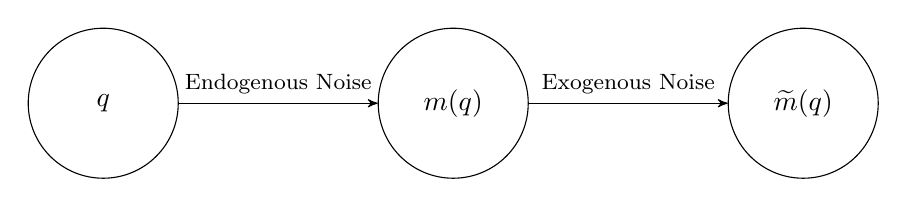
\begin{tikzpicture}[->,>=stealth',auto,node distance=1.75in,state/.style={circle,draw,minimum size=.75in}]
\node[state] (x0) {$q$};
\node[state] (x1) [right of=x0] {$m(q)$};
\node[state] (x2) [right of=x1] {$\widetilde{m}(q)$};
\draw[->] (x0) edge node[above]{\footnotesize Endogenous Noise} (x1);
\draw[->] (x1) edge node[above]{\footnotesize Exogenous Noise} (x2);
\end{tikzpicture}
\end{center}
\begin{itemize}
\item Discretizing $\downarrow$ \underline{exogenous} noise, but $\uparrow$ \underline{endogenous} noise.
\item In our setting, exogenous noise costs more than endogenous noise. 
\item Is our result robust?
\item\textbf{Proposition 2.} If 
\begin{enumerate} 
\item the noise is \underline{not} uniformly distributed, and 
\item the noise variance is sufficiently small, 
\end{enumerate}
then discrete messages are \underline{not} optimal. 
\end{itemize}
\end{frame}

%%%%%%%%%%%%%%%%%%
%%% CONCLUSION %%%
%%%%%%%%%%%%%%%%%%
\begin{frame}{Conclusion}
\begin{enumerate}
\item Discretization can be optimal, \textit{even} when sender's and receiver's interests are aligned.
\item While coarse messages are less precise, they are easier to interpret.
\item Continuous messages are optimal when the error is "small."
\item Rethink classic problems with aligned interests and noisy communication.
\end{enumerate}
\end{frame}

\end{document}